% Options for packages loaded elsewhere
\PassOptionsToPackage{unicode}{hyperref}
\PassOptionsToPackage{hyphens}{url}
%
\documentclass[
  ignorenonframetext,
]{beamer}
\usepackage{pgfpages}
\setbeamertemplate{caption}[numbered]
\setbeamertemplate{caption label separator}{: }
\setbeamercolor{caption name}{fg=normal text.fg}
\beamertemplatenavigationsymbolsempty
% Prevent slide breaks in the middle of a paragraph
\widowpenalties 1 10000
\raggedbottom
\setbeamertemplate{part page}{
  \centering
  \begin{beamercolorbox}[sep=16pt,center]{part title}
    \usebeamerfont{part title}\insertpart\par
  \end{beamercolorbox}
}
\setbeamertemplate{section page}{
  \centering
  \begin{beamercolorbox}[sep=12pt,center]{part title}
    \usebeamerfont{section title}\insertsection\par
  \end{beamercolorbox}
}
\setbeamertemplate{subsection page}{
  \centering
  \begin{beamercolorbox}[sep=8pt,center]{part title}
    \usebeamerfont{subsection title}\insertsubsection\par
  \end{beamercolorbox}
}
\AtBeginPart{
  \frame{\partpage}
}
\AtBeginSection{
  \ifbibliography
  \else
    \frame{\sectionpage}
  \fi
}
\AtBeginSubsection{
  \frame{\subsectionpage}
}

\usepackage{amsmath,amssymb}
\usepackage{iftex}
\ifPDFTeX
  \usepackage[T1]{fontenc}
  \usepackage[utf8]{inputenc}
  \usepackage{textcomp} % provide euro and other symbols
\else % if luatex or xetex
  \usepackage{unicode-math}
  \defaultfontfeatures{Scale=MatchLowercase}
  \defaultfontfeatures[\rmfamily]{Ligatures=TeX,Scale=1}
\fi
\usepackage{lmodern}
\ifPDFTeX\else  
    % xetex/luatex font selection
\fi
% Use upquote if available, for straight quotes in verbatim environments
\IfFileExists{upquote.sty}{\usepackage{upquote}}{}
\IfFileExists{microtype.sty}{% use microtype if available
  \usepackage[]{microtype}
  \UseMicrotypeSet[protrusion]{basicmath} % disable protrusion for tt fonts
}{}
\makeatletter
\@ifundefined{KOMAClassName}{% if non-KOMA class
  \IfFileExists{parskip.sty}{%
    \usepackage{parskip}
  }{% else
    \setlength{\parindent}{0pt}
    \setlength{\parskip}{6pt plus 2pt minus 1pt}}
}{% if KOMA class
  \KOMAoptions{parskip=half}}
\makeatother
\usepackage{xcolor}
\newif\ifbibliography
\setlength{\emergencystretch}{3em} % prevent overfull lines
\setcounter{secnumdepth}{-\maxdimen} % remove section numbering


\providecommand{\tightlist}{%
  \setlength{\itemsep}{0pt}\setlength{\parskip}{0pt}}\usepackage{longtable,booktabs,array}
\usepackage{calc} % for calculating minipage widths
\usepackage{caption}
% Make caption package work with longtable
\makeatletter
\def\fnum@table{\tablename~\thetable}
\makeatother
\usepackage{graphicx}
\makeatletter
\def\maxwidth{\ifdim\Gin@nat@width>\linewidth\linewidth\else\Gin@nat@width\fi}
\def\maxheight{\ifdim\Gin@nat@height>\textheight\textheight\else\Gin@nat@height\fi}
\makeatother
% Scale images if necessary, so that they will not overflow the page
% margins by default, and it is still possible to overwrite the defaults
% using explicit options in \includegraphics[width, height, ...]{}
\setkeys{Gin}{width=\maxwidth,height=\maxheight,keepaspectratio}
% Set default figure placement to htbp
\makeatletter
\def\fps@figure{htbp}
\makeatother
% definitions for citeproc citations
\NewDocumentCommand\citeproctext{}{}
\NewDocumentCommand\citeproc{mm}{%
  \begingroup\def\citeproctext{#2}\cite{#1}\endgroup}
\makeatletter
 % allow citations to break across lines
 \let\@cite@ofmt\@firstofone
 % avoid brackets around text for \cite:
 \def\@biblabel#1{}
 \def\@cite#1#2{{#1\if@tempswa , #2\fi}}
\makeatother
\newlength{\cslhangindent}
\setlength{\cslhangindent}{1.5em}
\newlength{\csllabelwidth}
\setlength{\csllabelwidth}{3em}
\newenvironment{CSLReferences}[2] % #1 hanging-indent, #2 entry-spacing
 {\begin{list}{}{%
  \setlength{\itemindent}{0pt}
  \setlength{\leftmargin}{0pt}
  \setlength{\parsep}{0pt}
  % turn on hanging indent if param 1 is 1
  \ifodd #1
   \setlength{\leftmargin}{\cslhangindent}
   \setlength{\itemindent}{-1\cslhangindent}
  \fi
  % set entry spacing
  \setlength{\itemsep}{#2\baselineskip}}}
 {\end{list}}
\usepackage{calc}
\newcommand{\CSLBlock}[1]{\hfill\break\parbox[t]{\linewidth}{\strut\ignorespaces#1\strut}}
\newcommand{\CSLLeftMargin}[1]{\parbox[t]{\csllabelwidth}{\strut#1\strut}}
\newcommand{\CSLRightInline}[1]{\parbox[t]{\linewidth - \csllabelwidth}{\strut#1\strut}}
\newcommand{\CSLIndent}[1]{\hspace{\cslhangindent}#1}

\makeatletter
\@ifpackageloaded{caption}{}{\usepackage{caption}}
\AtBeginDocument{%
\ifdefined\contentsname
  \renewcommand*\contentsname{Table of contents}
\else
  \newcommand\contentsname{Table of contents}
\fi
\ifdefined\listfigurename
  \renewcommand*\listfigurename{List of Figures}
\else
  \newcommand\listfigurename{List of Figures}
\fi
\ifdefined\listtablename
  \renewcommand*\listtablename{List of Tables}
\else
  \newcommand\listtablename{List of Tables}
\fi
\ifdefined\figurename
  \renewcommand*\figurename{Figure}
\else
  \newcommand\figurename{Figure}
\fi
\ifdefined\tablename
  \renewcommand*\tablename{Table}
\else
  \newcommand\tablename{Table}
\fi
}
\@ifpackageloaded{float}{}{\usepackage{float}}
\floatstyle{ruled}
\@ifundefined{c@chapter}{\newfloat{codelisting}{h}{lop}}{\newfloat{codelisting}{h}{lop}[chapter]}
\floatname{codelisting}{Listing}
\newcommand*\listoflistings{\listof{codelisting}{List of Listings}}
\makeatother
\makeatletter
\makeatother
\makeatletter
\@ifpackageloaded{caption}{}{\usepackage{caption}}
\@ifpackageloaded{subcaption}{}{\usepackage{subcaption}}
\makeatother
\ifLuaTeX
  \usepackage{selnolig}  % disable illegal ligatures
\fi
\usepackage{bookmark}

\IfFileExists{xurl.sty}{\usepackage{xurl}}{} % add URL line breaks if available
\urlstyle{same} % disable monospaced font for URLs
\hypersetup{
  pdftitle={Relative price dispersion and inflation regimes in South Africa},
  pdfauthor={Keagile Lesame and Xolani Sibande},
  hidelinks,
  pdfcreator={LaTeX via pandoc}}

\title{Relative price dispersion and inflation regimes in South Africa}
\author{Keagile Lesame and Xolani Sibande}
\date{}

\begin{document}
\frame{\titlepage}

\section{Motivation}\label{motivation}

\begin{frame}{Motivation}
\phantomsection\label{motivation-1}
\end{frame}

\section{Literature}\label{literature}

\begin{frame}{Relative price dispersion through Lucas's aggregate supply
curve}
\phantomsection\label{relative-price-dispersion-through-lucass-aggregate-supply-curve}
\end{frame}

\begin{frame}{Empirical literaturer review}
\phantomsection\label{empirical-literaturer-review}
\end{frame}

\section{Data and methodology}\label{data-and-methodology}

\begin{frame}{Data}
\phantomsection\label{data}
Our analysis uses monthly inflation data on 45 goods categories from
January 2009 to November 2025 obtained from Statistics South Africa
(Stats SA).\footnote<.->{The data is available at:
  \url{http://www.statssa.gov.za/} The data is seasonally adjusted.} .
\textbf{?@fig-headline\_inflation} below shows the long term inflation
rate in South Africa, and \textbf{?@fig-price\_data} in the appendix
shows the various price categories used in the analysis.
\textbf{?@tbl-descriptive\_stats} provides the descriptive statistics of
the inflation rates for the various price categories used in the
analysis.
\end{frame}

\begin{frame}{Methodology}
\phantomsection\label{methodology}
The relative price dispersion (RPD) is calculated in line with @lach1992
as the weighted standard deviation of individual price inflation rates
from the aggregate inflation rate. The RPD is essentially the
variability of relative prices of a given product. We first calculate
the monthly inflation rate as follows:

\begin{equation}\phantomsection\label{eq-inflation_rate}{ \pi_{i,t} = ln\left(\frac{P_{i,t}}{P_{i,t-1}}\right) * 100, }\end{equation}

where \(\pi_{i,t}\) is the inflation rate of good \(i\) at time \(t\),
\(P_{i,t}\) is the price of good \(i\) at time \(t\), and \(P_{i,t-1}\)
is the price of good \(i\) at time \(t-1\).
\end{frame}

\begin{frame}{Methodology}
\phantomsection\label{methodology-1}
Then, the RPD is calculated as:

\begin{equation}\phantomsection\label{eq-rpd}{RPD_{t} = \sqrt{\sum_{i=1}^{n}\omega_{i}(\pi_{i,t} - \pi_{t})^2}, }\end{equation}

where \(\omega_{j}\) is the expenditure share of the \(j^{th}\) good,
\(\pi_{t}\) is the headline or aggregate inflation rate at time \(t\),
and \(\sum_{i=1}^{n}\omega_{i} = 1\). The expenditure weights
(\(\omega_{i}\)) used are derived from the Consumer Price Index (CPI)
basket provided by Stats SA. Figure~\ref{fig-rpd} shows the RPD
calculated using the above formula. We use the 2025 CPI Stats SA
weights. The weights are shown in \textbf{?@fig-weights} in the
appendix.
\end{frame}

\begin{frame}{Methodology}
\phantomsection\label{methodology-2}
To examine the relationship between inflation and RPD, we estimate the
following econometric model:

\begin{equation}\phantomsection\label{eq-rpd_reg}{RPD_{t} = \beta_0 + \beta_1|\pi_{t}| + \sum_{h=1}^{3}\omega_hRPD_{t-h}  +  \mu_{t}, }\end{equation}

where \(RPD_{t}\) is the relative price variance at time \(t\),
\(|\pi_{t}|\) is the absolute value of aggregate inflation rate at time
\(t\), \(RPD_{t-h}\) are lagged values of RPD to account for its dynamic
nature, and \(\mu_{t}\) is the error term. The coefficient \(\beta_1\)
captures the effect of inflation on RPD. We include three lags of RPD
based on Akaike Information Criterion (AIC) (and other tests) and to
capture potential persistence in RPD. For robustness, we repeat this
estimation using core inflation (excluding food and non-alcoholic
beverages, and fuel and electricity) instead of headline inflation to
account for the potential volatility in these components.
\end{frame}

\begin{frame}{Methodology}
\phantomsection\label{methodology-3}
The literature on RPD emphasises that the relationship between inflation
and RPD maybe time-varying due to structural changes in the economy,
monetary policy regimes, and other factors. To capture potential time
variation in the relationship, we also estimate a rolling regression
model with a 24-month and 60-month windows as follows:

\begin{equation}\phantomsection\label{eq-rpd_rolling_reg}{RPD_{t} = \alpha_{t} + \beta_{1,t}|\pi_{t}| + \sum_{h=1}^{3}\omega_{h,t}RPD_{t-h}  +  \mu_{t}, }\end{equation}

where the coefficients \(\alpha_{t}\), \(\beta_{1,t}\), and
\(\omega_{h,t}\) vary over time. This approach allows us to observe the
stability of the coefficients over time, which is an indicator of
non-linearity in the relationship between RPD and inflation.
\end{frame}

\begin{frame}{Methodology}
\phantomsection\label{methodology-4}
Next, we utilise a semi-parametric or partially linear approach to
estimate the optimal level of inflation given the RPD. This approach
allows us to model the relationship between inflation and RPD without
imposing a strict functional form. Following the literature, we first
specify a quadratic (U-shaped) relationship between inflation and RPD as
follows:

\begin{equation}\phantomsection\label{eq-rpd_semi_parametric}{RPD_t = \alpha + \pi_t + \beta_2\pi_t^2 + \sum_{h=1}^{3}\phi_hRPD_{t-h} + \epsilon_t, }\end{equation}

where \(\beta_2\) captures the curvature of the relationship between
inflation and RPD. The optimal inflation rate that minimizes RPD can be
derived by taking the first derivative of the equation with respect to
\(\pi_t\) and setting it to zero, yielding:

\begin{equation}\phantomsection\label{eq-optimal_inflation}{\pi_t^* = -\dfrac{1}{2\beta_2}.}\end{equation}
\end{frame}

\begin{frame}{Methodology}
\phantomsection\label{methodology-5}
To estimate this optiomal inflation we implement a semi parametric
approach as follows:

\begin{equation}\phantomsection\label{eq-rpd_semi_parametric_f}{RPD_t =  f(\pi_t) + \sum_{h=1}^{3}\phi_hRPD_{t-h} + \epsilon_t, }\end{equation}

where \(f(\pi_t)\) is a non-linear smooth differentiable function of
inflation and the RPD. Therefore, the optimal inflation rate can be
obtained by finding the minimum of the estimated \(f(\pi_t)\) function.
\(f(\pi_t)\) is estimated in two stages. First we estimate \(\lambda_h\)
as follows:

\begin{equation}\phantomsection\label{eq-rpd_semi_parametric_stage1}{ RPD_t = \sum_{h=1}^{3}\lambda_h\overline{RPD}_{t-h} + \eta_t, }\end{equation}

where \(\overline{RPD}_{t-h}\) are the residuals from a non-parametric
regression of each lag of \(RPD_t\) on \(\pi_t\). In the second stage,
we estimate \(f(\pi_t)\) non-parametrically as follows:

\begin{equation}\phantomsection\label{eq-rpd_semi_parametric_stage2}{\hat{\eta}_t = f(\pi_t) + v_t, }\end{equation}

where \(\hat{\eta}_t\) are the residuals from
Equation~\ref{eq-rpd_semi_parametric_stage1}, and \(f(\pi_t)\) is
estimated using a kernel regression method. The bandwidth (\(h\)) for
the kernel estimator is selected using cross-validation to minimize the
mean squared error. As a treatment for extreme values of inflation, we
further implement the unbounded Gaussian kernel and the outlier-robust
Epanechnikov kernel. In essence, the semi-parametric approach captures
the sensitivity of RPD to marginal increases in inflation. In that case,
the optimal inflation rate can be obtained by finding the point where
the first derivative (\(f'(\pi_t)\)) is equal to zero. Therefore, if
\(f'(\pi_t) > 0\) (\(f'(\pi_t) < 0\)), then an increase in inflation
(decrease) leads to an increase (decrease) in the RPD. For robustness we
estimate the \(g(UIN_t)\) with multiple bandwith (\(h\)).
\end{frame}

\begin{frame}{Methodology}
\phantomsection\label{methodology-6}
To further disentangle the effects of RPD on inflation, we decompose
headline inflation into its expected and unexpected components. As
discussed in the literature section, for example, theory suggests that
inflation uncertainty has a more pronounced effect on RPD due to
information frictions faced by firms when adjusting prices
{[}@lucas1973; @hercowitz1981; @cukierman1983{]}.

We therefore estimate the following model:

\begin{equation}\phantomsection\label{eq-unexpected}{ RPD_t = \alpha + \beta_0 EIN_t + \beta_1 UIN_t + g(UIN_t) + \sum_{k=1}^{3}\lambda_k RPD_{t-k} + \epsilon_t, }\end{equation}

where \(EIN_t\) is the expected inflation rate, \(UIN_t\) is the
unexpected inflation rate, and \(g(UIN_t)\) is a non-linear function of
unexpected inflation (\(UIN_t\)). We obtain the expected using \textbf{a
simple moving average of headline inflation, and unexpected inflation as
the standard deviation of inflation}. The estimation of \(g(UIN_t)\)
follows the same two-stage semi-parametric approach outlined in
Equation~\ref{eq-rpd_semi_parametric_stage1} and
Equation~\ref{eq-rpd_semi_parametric_stage2}. The number of lags is the
same as in Equation~\ref{eq-rpd_reg}.

Lastly, and some-what novel to the RPD literature, we employ a quantile
on quantile regression approach {[}@koenker2017{]}. Quantile on quantile
regressions are robust to outliers and allows us to estimate the regime
aspects of the relationship between RPD and inflation. For brevity, we
explain the quantile on quantile estimation procedure in the Appendix.
\end{frame}

\section{Results}\label{results}

\begin{frame}{Results}
\phantomsection\label{results-1}
\begin{figure}[H]

\centering{

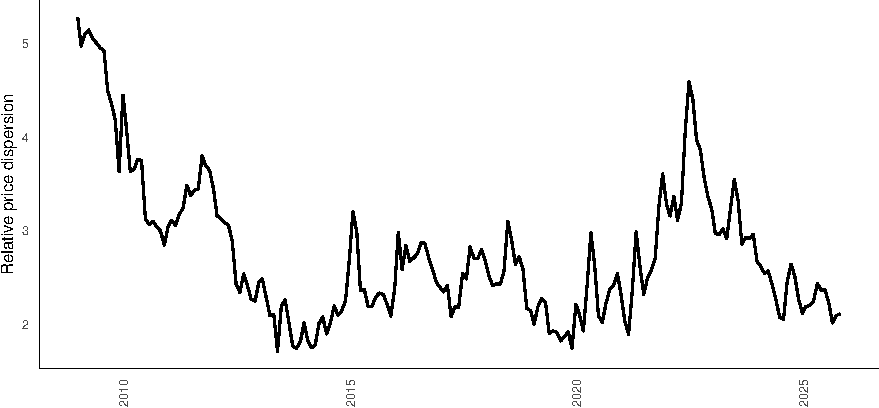
\includegraphics{inflation_relative_price_variance_presentation_files/figure-beamer/fig-rpd-1.pdf}

}

\caption{\label{fig-rpd}RPD over-time}

\end{figure}%
\end{frame}

\begin{frame}{Results}
\phantomsection\label{results-2}
\begin{figure}[H]

\centering{

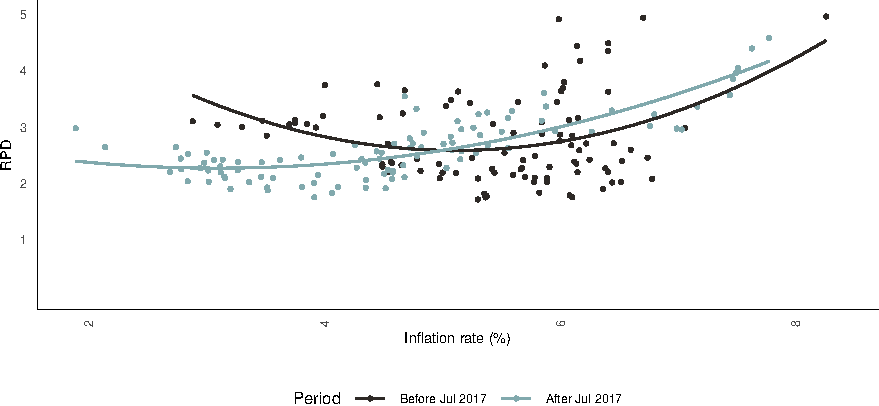
\includegraphics{inflation_relative_price_variance_presentation_files/figure-beamer/fig-rpd_inflation-1.pdf}

}

\caption{\label{fig-rpd_inflation}RPD vs headline Inflation}

\end{figure}%
\end{frame}

\begin{frame}{Results}
\phantomsection\label{results-3}
\begin{figure}[H]

\centering{

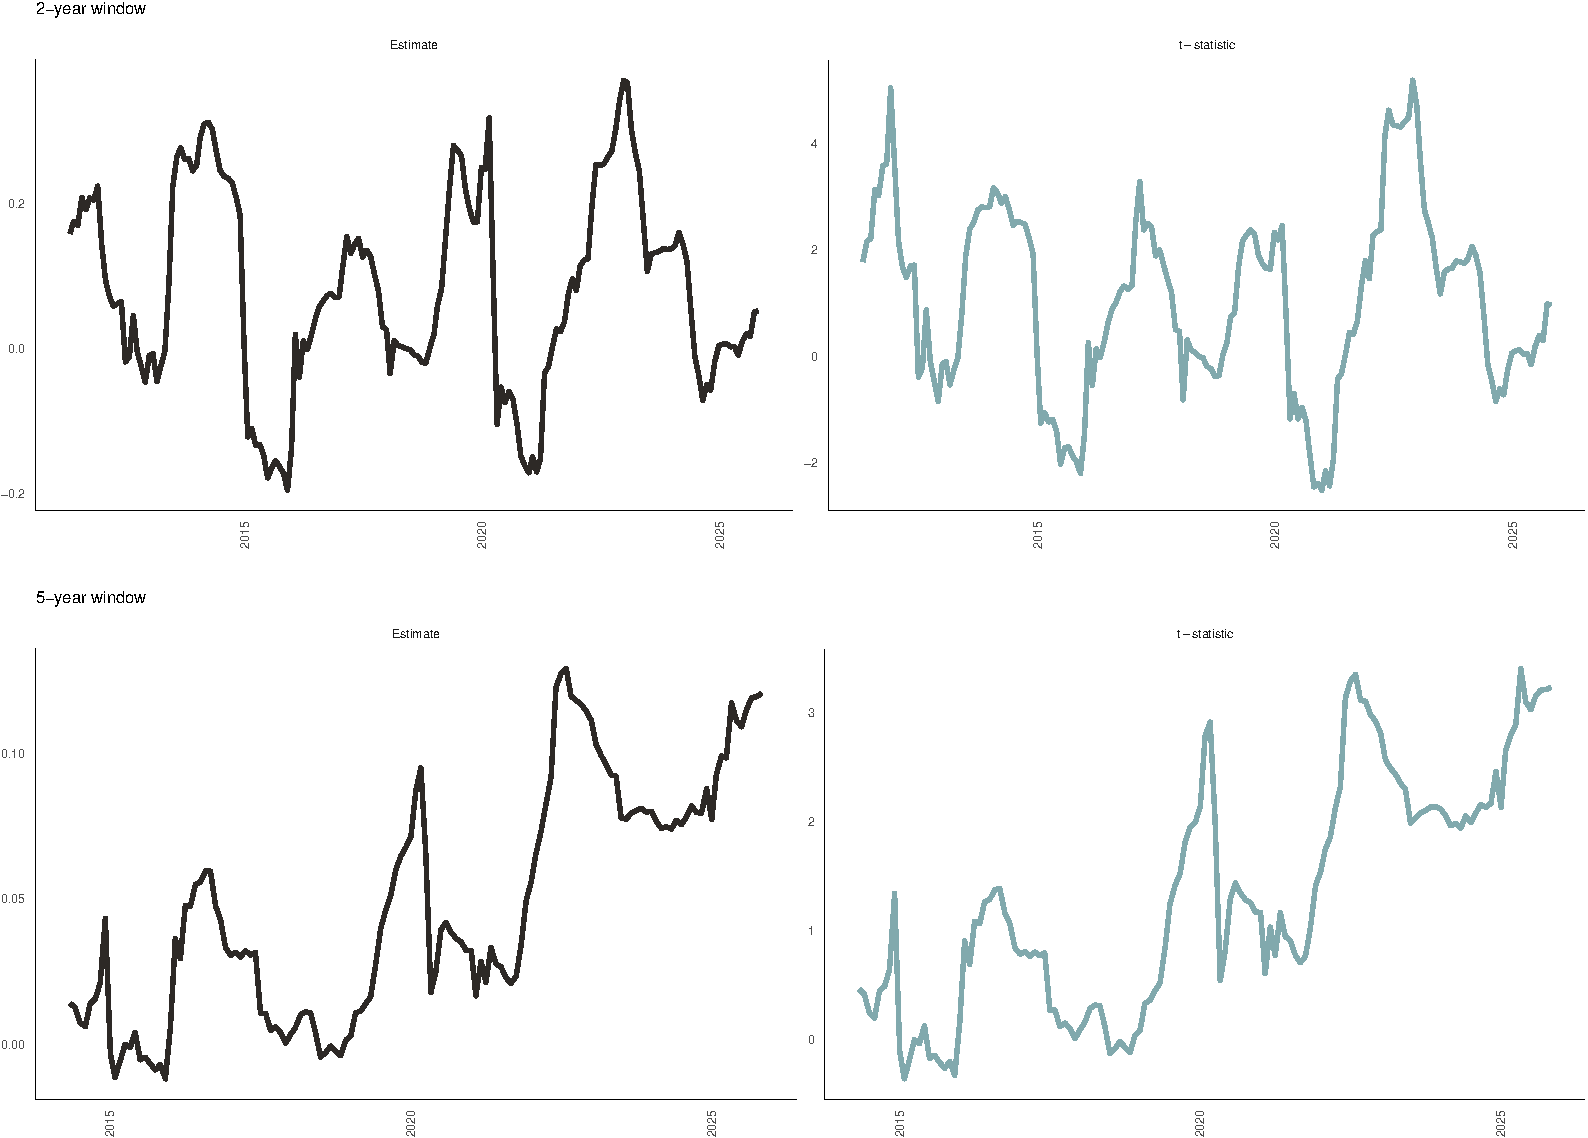
\includegraphics{inflation_relative_price_variance_presentation_files/figure-beamer/fig-rolling_coefficients-1.pdf}

}

\caption{\label{fig-rolling_coefficients}Rolling regressions. Note:
t-statistics of greater (or less) than 1.96 ( or -1.96) is sigficant at
a 5\% level of significance.}

\end{figure}%
\end{frame}

\begin{frame}{Results}
\phantomsection\label{results-4}
\begin{figure}[H]

\centering{

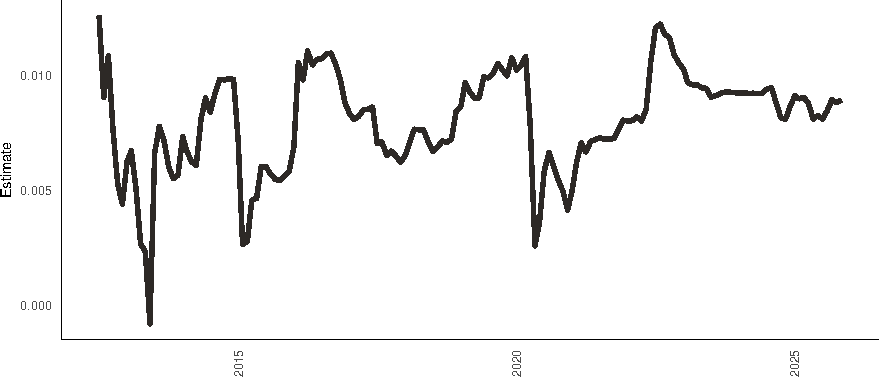
\includegraphics{inflation_relative_price_variance_presentation_files/figure-beamer/fig-recursive-1.pdf}

}

\caption{\label{fig-recursive}Recursive regressions. Note: Recursive
regression estimates of the coefficient on absolute headline inflation
with a fixed start date of 2012-07.}

\end{figure}%
\end{frame}

\begin{frame}{Results}
\phantomsection\label{results-5}
\begin{figure}[H]

\centering{

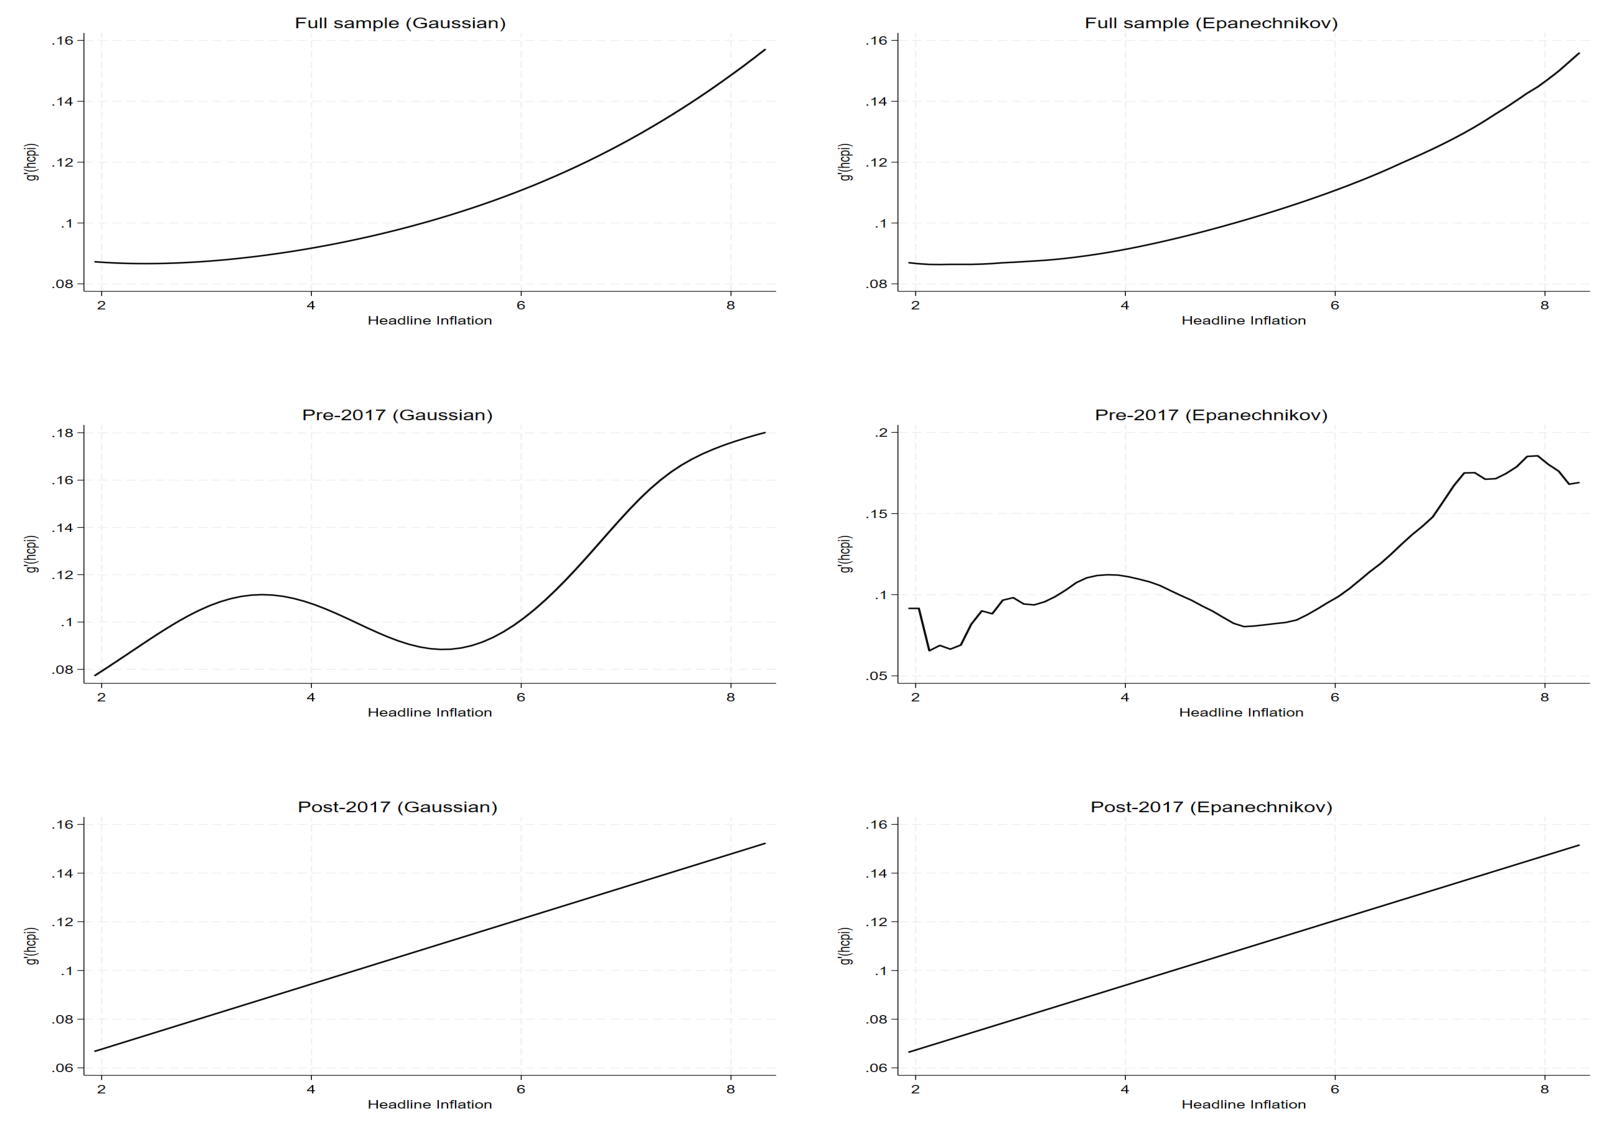
\includegraphics{inflation_relative_price_variance_presentation_files/figure-beamer/fig-semi_parametric-1.pdf}

}

\caption{\label{fig-semi_parametric}Semi-parametric regressions}

\end{figure}%
\end{frame}

\begin{frame}{Results}
\phantomsection\label{results-6}
\begin{figure}[H]

\centering{

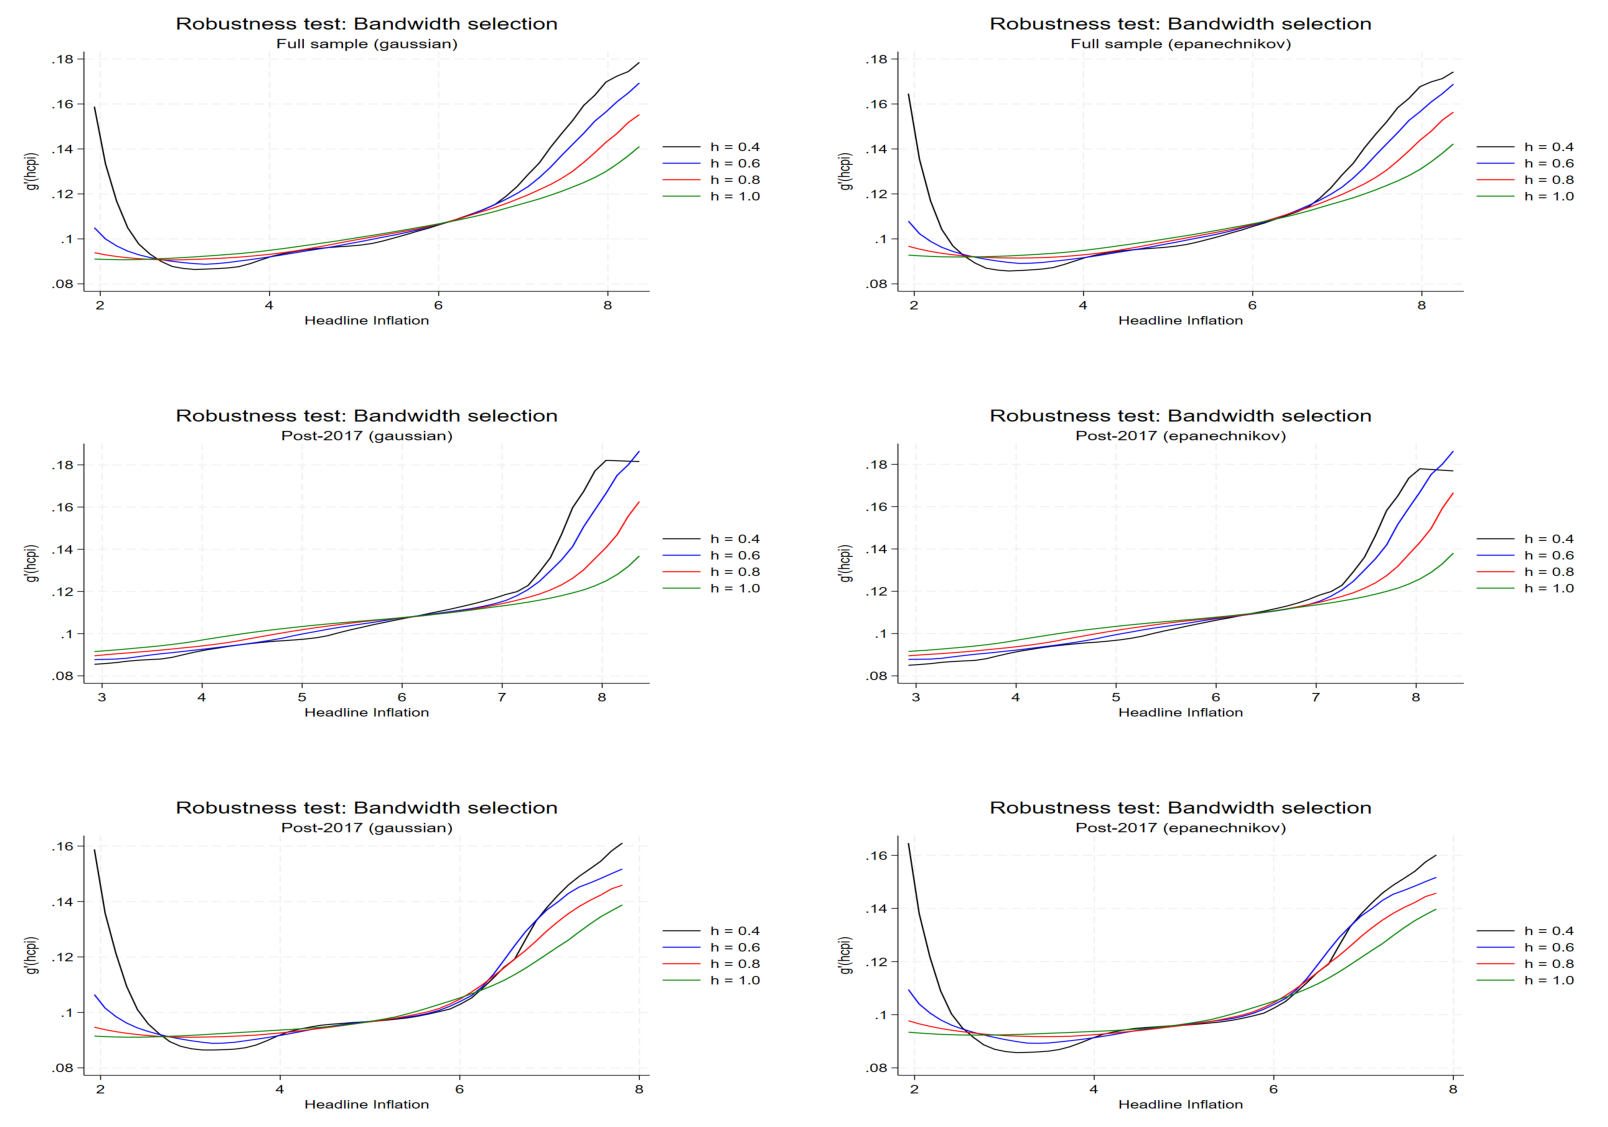
\includegraphics{inflation_relative_price_variance_presentation_files/figure-beamer/fig-semi_parametric_robustness-1.pdf}

}

\caption{\label{fig-semi_parametric_robustness}Semi-parametric
regressions with alternative bandwidth selection. Note: hcpi is the
headline inflation rate.}

\end{figure}%
\end{frame}

\begin{frame}{Results}
\phantomsection\label{results-7}
\begin{figure}[H]

\centering{

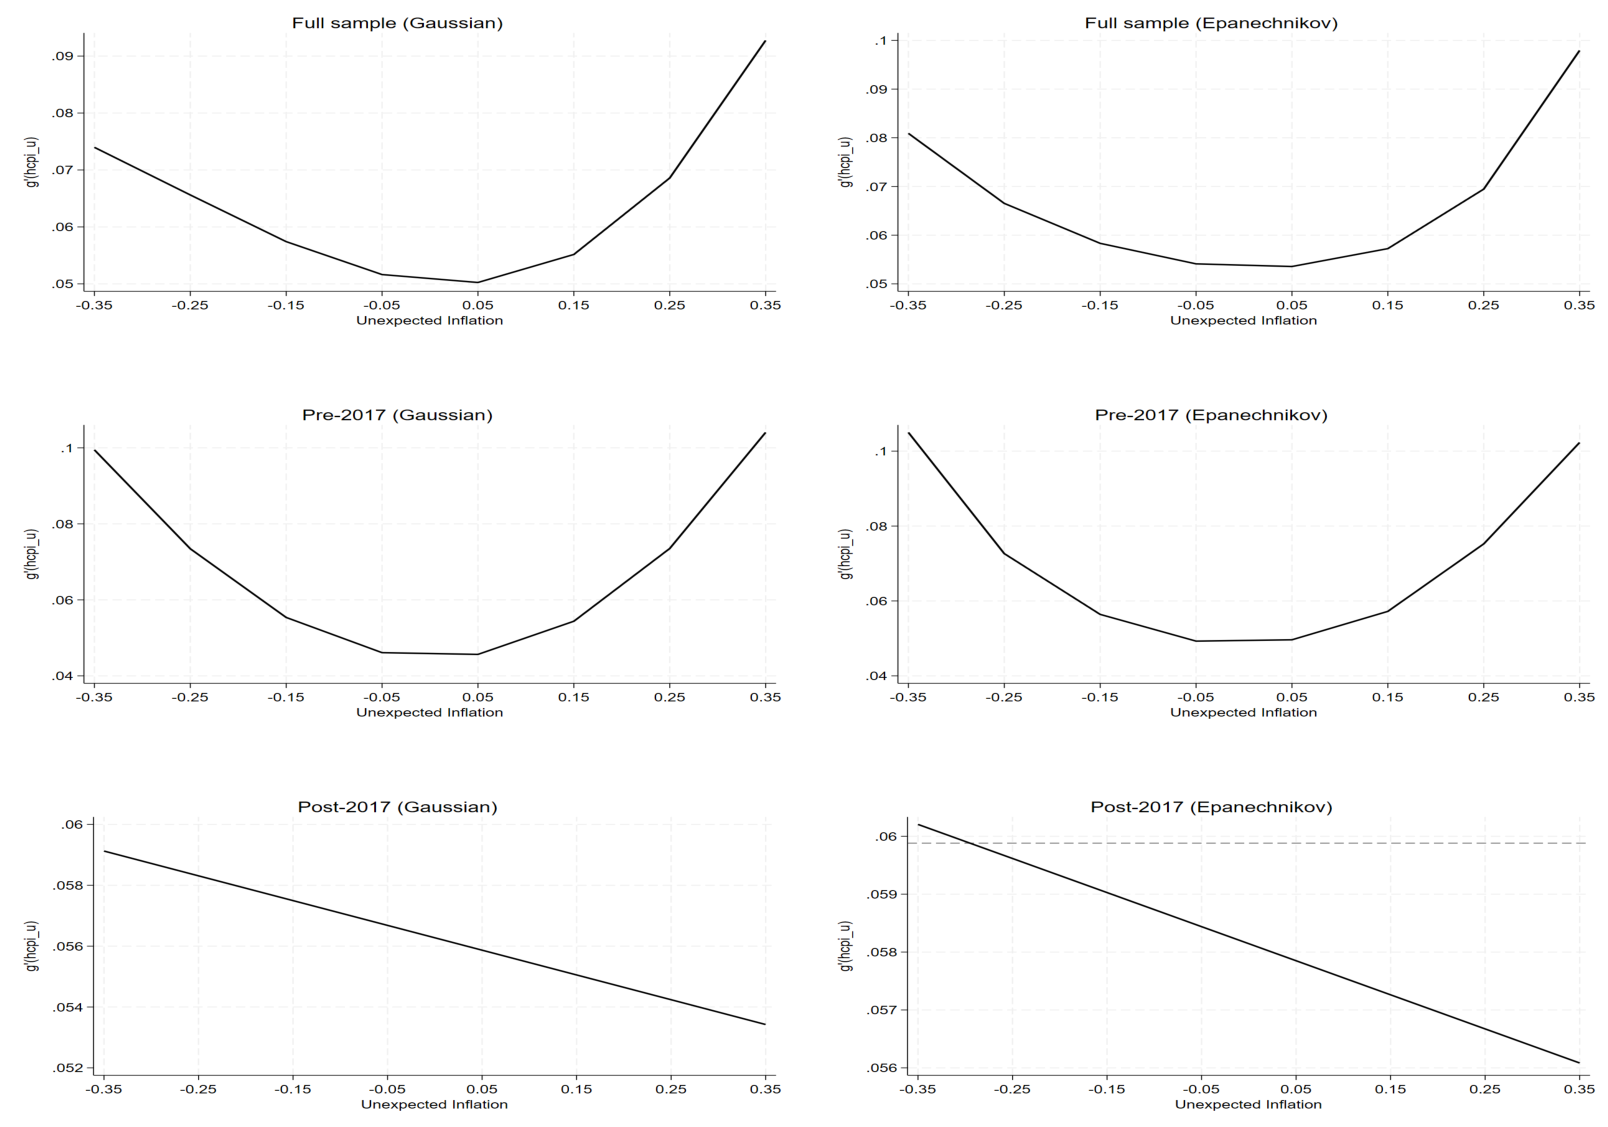
\includegraphics{inflation_relative_price_variance_presentation_files/figure-beamer/fig-unexpected_inflation-1.pdf}

}

\caption{\label{fig-unexpected_inflation}Semi-parametric regressions for
unexpected inflation. Note: hcpi\_u is the unexpected component of
headline inflation.}

\end{figure}%
\end{frame}

\begin{frame}{Results}
\phantomsection\label{results-8}
\begin{figure}[H]

\centering{

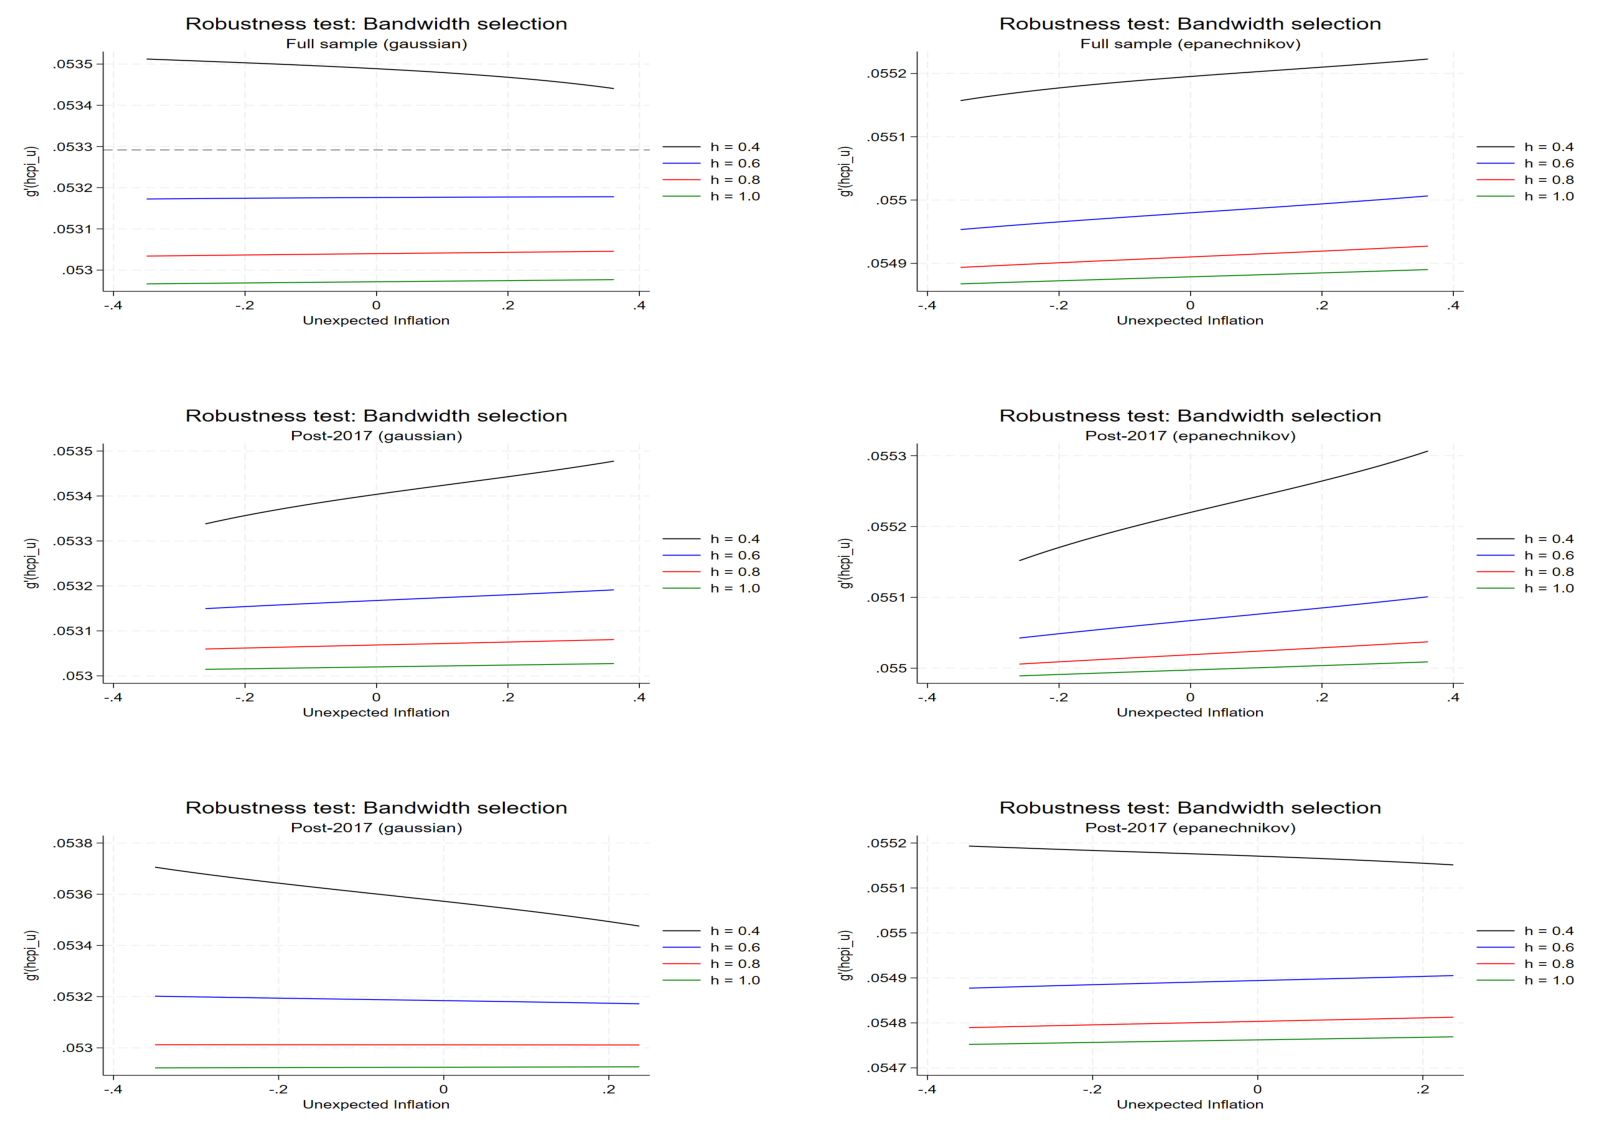
\includegraphics{inflation_relative_price_variance_presentation_files/figure-beamer/fig-semi_parametric_unexpected_robustness-1.pdf}

}

\caption{\label{fig-semi_parametric_unexpected_robustness}Semi-parametric
regressions for unexpected inflation with alternative bandwidth
selection. Note: hcpi\_u is the unexpected component of headline
inflation.}

\end{figure}%
\end{frame}

\begin{frame}{Results}
\phantomsection\label{results-9}
\begin{figure}[H]

\centering{

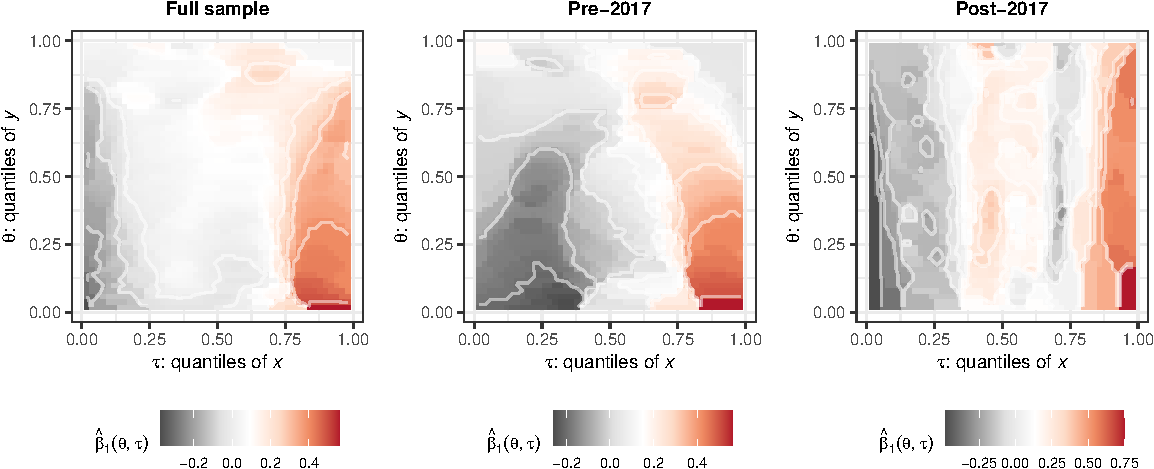
\includegraphics{inflation_relative_price_variance_presentation_files/figure-beamer/fig-quant_reg-1.pdf}

}

\caption{\label{fig-quant_reg}Quantile on quantile regressions for
headline inflation. Note: In the quantile on quatile regression plots,
the x-axis represents the quantiles of headline inflation, while the
y-axis represents the quantiles of RPD. The color gradient indicates the
strength and direction of the relationship between headline inflation
and RPD across different quantiles. Warmer colors (e.g., red) indicate a
stronger positive relationship, while cooler colors (e.g., blue)
indicate a stronger negative relationship. The white areas represent
quantiles where the relationship is not statistically significant.}

\end{figure}%
\end{frame}

\begin{frame}{Results}
\phantomsection\label{results-10}
\begin{figure}[H]

\centering{

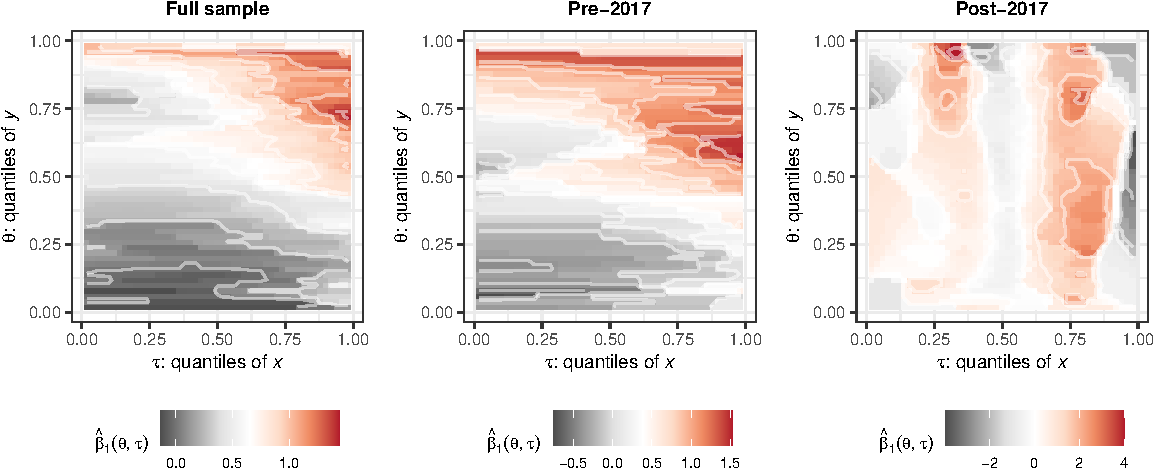
\includegraphics{inflation_relative_price_variance_presentation_files/figure-beamer/fig-unif_quant_reg-1.pdf}

}

\caption{\label{fig-unif_quant_reg}Quantile on quantile regressions for
the unexpected componenet of inflation. Note: The x-axis represents the
quantiles of the unexpected componenet of headline inflation, while the
y-axis represents the quantiles of RPD.}

\end{figure}%
\end{frame}

\section{Conclusions}\label{conclusions}

\begin{frame}{Conclusion}
\phantomsection\label{conclusion}
\end{frame}

\begin{frame}{References}
\phantomsection\label{references}
\phantomsection\label{refs}
\begin{CSLReferences}{0}{1}
\end{CSLReferences}
\end{frame}



\end{document}
